\documentclass[11pt]{report}
\setlength{\topmargin}{-.5in}
\setlength{\textheight}{9in}
\setlength{\oddsidemargin}{.125in}
\setlength{\textwidth}{6.25in}
\usepackage{hyperref}
\usepackage{graphicx}
\pagestyle{plain}

\begin{document}

\title{JokeOfTheDay}
\author{Aniket Pansare, Sagar Abhang}
\maketitle
\begin{abstract}
JokeOfTheDay is an application developed in Android which allows the user to get his current location along with a joke for that day. The application makes use of the Android's Location Manager Services for fetching the user location based on the GPS provider and Network Provider. It selects the best provider among the available providers on the basis of criteria specified. The location information is retrieved using the latitude and longitude. The Application makes a TCP connection to the “impact.asu.edu” server to fetch the joke of the day. It performs a proper handshake with the server in a predefined message format and retrieves the Joke of the Day. After receiving the Joke, the application displays the joke on the screen and gracefully closes the connection with the server.
\end{abstract}
\tableofcontents
\newpage

\section{Purpose of the Assignment:}
To design an Android application, that makes use of location services and client-server programming. The main focus of this assignment is for students to get familiar with the android framework.

\section{Software Requirement and Specifications}
\subsection{Major Constraints:}
\begin{enumerate}
\item The Application will run only on android powered devices.
\item The device must have GPS and Internet access for location information to be displayed along with the joke.
\item The http://impact.asu.edu:8000 server must be up and running to display the Joke of the Day.
\end{enumerate}

\subsection{Hardware Resources used:}
\begin{itemize}
\item Android powered Mobile device or Tablet.
\item RAM 256MB
\item Processor: 600Mhz, MSM7227, Qualcomm
\end{itemize}

\subsection{Software Resources used:}
\begin{itemize}
\item Android 1.6 SDK, Release 1
\item Platform: Android 2.2,Froyo
\item Eclipse SDK: Juno
\item JDK 1.7.0\_07
\end{itemize}	

\section{Technical Details:}
\begin{itemize}
\item User-permissions: INTERNET and ACCESS\_FINE\_LOCATION permissions given in AndroidManifest.xml
\item Package: com.example.jokeoftheday
\item Source files: \begin{enumerate}
                            \item MainActivity.java
                            \item ConnectGetThread.java
                    \end{enumerate}
\item xml files:  activity\_main.xml
\item Executable File: JokeOfTheDay.apk
\end{itemize}

\section{Design and Implementation:}
The JokeOfTheDay application displays a joke on the user\symbol{'40}s request. It also makes use of the Location services provided on the Android platform to determine the current location of the user and displays it on the screen.
\\[11pt ]The Joke server is hosted at “impact.asu.edu” and port 8000. The application acts as client and connects to Joke server via TCP connection. The application follows a predefined syntax to communicate with the server and fetch the joke of the day.
\\[11pt ]We used the request and response format, so that messages sent and received are parsed properly on both client and server side. Multiple contiguous spaces to separate fields not allowed, we used just one space character to separate the fields in message.

\section*{Request and Response format:}
Format: \textless AA1 MSGTYPE WHO WHAT \textgreater
\begin{itemize}
\item with MSGTYPE being HELLO THIS IS, HI, GOODBYE, REQUEST, RESPONSE;
\item with WHO being the server name or client name;
\item with WHAT being what is being communicated with the MSGTYPE. (WHAT may be empty)
\end{itemize}

\section*{Message Parsing:}
The application establishes a socket connection with the server and waits for server to respond. The server responds in pre-defined syntax, such as \textless aa1 msgtype who what\textgreater. The request from the server is parsed till the end of the message i.e \textgreater is received. To do message parsing java class StringBuffer is used as it is more efficient than class String.
\begin{enumerate}
\item Server: \textless AA1 HELLO THIS IS servername WHO ARE YOU?\textgreater
\item Client: \textless AA1 HELLO THIS IS clientname\textgreater
\item Server: \textless AA1 HI clientname PLEASE SEND YOUR REQUEST\textgreater
\item Client: \textless AA1 REQUEST servername JOTD\textgreater
\item Server: \textless AA1 RESPONSE clientname JOTD joke\_of\_the\_day\_text\textgreater
\item Client: \textless AA1 GOODBYE servername\textgreater
\item Server: \textless AA1 GOODBYE clientname HAVE A NICE DAY\textgreater
\end{enumerate}	

\section*{Criteria:}
We used the method getBestProvider(Criteria criteria, boolean enabledOnly) to fetch the location provider that best meets the given criteria. If several providers meet the criteria, then one with the best accuracy is returned.
\\[11pt]Following criteria is set for getting the Best Provider.
\begin{itemize}
\item Accuracy: ACCURACY\_FINE   (To get finer location accuracy)
\item Altitude Required: True    (Provider with altitude information)
\item Bearing Required: True     (Provider with bearing information)
\item Cost Allowed: True         (Provider allowed to incur monetary cost)
\item Power Required: POWER\_LOW (To get provider with low power requirement)
\end{itemize}

\section*{Threading:}
Initially we tried implementing the joke fetching code in the main thread. But the Honeycomb SDK and above versions does not allow networking operations in main thread.It recommends the use of a separate thread[1]. So we created a separate thread to fetch the joke from Joke Server. Threading also helps to capture the on location change event updates and display it on the screen.

\section*{Scrollbar:}
TextView widget is used to display the joke received from server. If the joke has multiple lines, then only few lines of the joke were getting displayed. To address this issue, we used the scroll bar to display the Joke of the day. This allows the user to scroll in case the joke has multiple lines or the application is used on a device having smaller screen.

\section*{Log:}
To keep track of what is happening in the background when application is running, we used android.util.Log API to log the output.

\section{Limitations}
\begin{enumerate}
\item The client does not time out even if server does not send anything for certain time. The client needs to specify timeout period for which client waits for response from server.
\item Device must have GPS enabled to get location.
\end{enumerate}

\section{Future work}
\begin{enumerate}
\item Google maps can be used to display location of the user.
\item Timeout functionality is to be implemented so that client does not wait for indefinite time for server’s response.
\end{enumerate}

\section{Conclusion}
JokeOfTheDay application is implemented on Android SDK. On the technical perspective, using of Android API to get location of the user is very efficient than writing new one. Use of Java Multithreading concept improves the responsiveness of the application[2]. Future work can be done using Google Map API and project results can be verified on different locations.

\section{Application Run}
\begin{figure}[htp]
\label{fig:img1}
\caption{JokeOfTheDay in Applications.}
\centerline{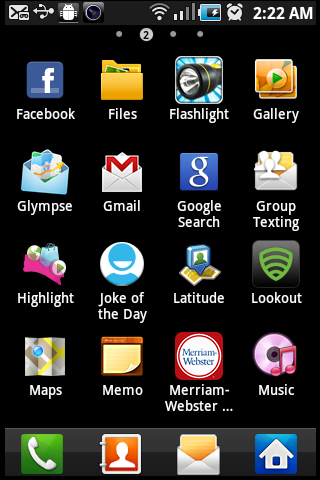
\includegraphics[scale=0.6]{1_JokeOfTheDay_in_APPLICATIONS}}
\end{figure}
\begin{figure}
\label{fig:img2}
\caption{JokeOfTheDay Application On Launch}
\centerline{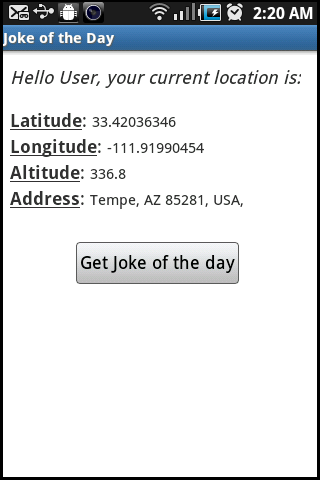
\includegraphics[scale=0.6]{2_Launched_JokeOfTheDay_Application}}
\end{figure}
\begin{figure}
\label{fig:img3}
\caption{JokeOfTheDay Application Output}
\centerline{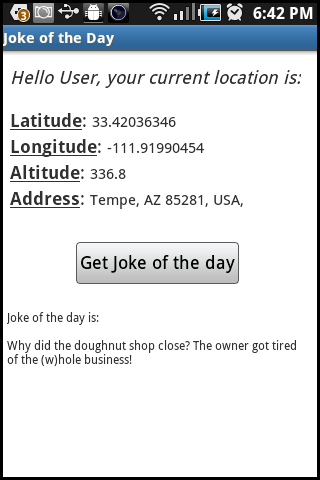
\includegraphics[scale=0.6]{3_Joke_Displayed_On_Screen}}
\end{figure}

\begin{thebibliography}{3}
\bibitem{} Developers: NetworkOnMainThreadException:
\\*[11pt] \url{http://developer.android.com/reference/android/os/NetworkOnMainThreadException.html},September 2012.
\bibitem{} Android Developers: Designing for Responsiveness:
\\*[11pt] \url{http://developer.android.com/guide/practices/responsiveness.html},September 2012.
\end{thebibliography}

\end{document}